% filepath: volunteer_hub_presentation.tex
\documentclass{beamer}

% Use a clean, professional theme
\usetheme{Madrid}
\usecolortheme{whale}
\useinnertheme{rectangles}
\useoutertheme{miniframes}

% Remove navigation symbols
\setbeamertemplate{navigation symbols}{}

% Add page numbers
\setbeamertemplate{footline}[frame number]

% Define colors
\definecolor{primarycolor}{RGB}{99, 102, 241}
\definecolor{secondarycolor}{RGB}{79, 70, 229}
\setbeamercolor{title}{fg=white,bg=primarycolor}
\setbeamercolor{frametitle}{fg=primarycolor,bg=white}
\setbeamercolor{structure}{fg=primarycolor}

% Packages
\usepackage{graphicx}
\usepackage{booktabs}
\usepackage{amsmath}
\usepackage{amsfonts}
\usepackage{amssymb}
\usepackage{listings}
\usepackage{xcolor}

% Title information
\title{\textbf{VolunteerHub: A Volunteer Management System}}
\subtitle{DBMS Mini Project}
\author{Adithya S (USN: 1BY23AI007) \\ Aditya B (USN: 1BY23AI009)}
\institute{Under the Guidance of\\
\textbf{Dr Archana Bhat}\\
Assistant Professor, Department of Artificial Intelligence\\ and Machine Learning\\
BMS Institute of Technology and Management}
\date{May 20, 2025}

\begin{document}

% Title slide
\begin{frame}
  \titlepage
\end{frame}

% Table of contents
\begin{frame}{Contents}
  \tableofcontents
\end{frame}

\section{Introduction}

\begin{frame}{Abstract}
  \begin{block}{Project Overview}
    VolunteerHub is a comprehensive web-based volunteer management system designed to streamline the process of organizing volunteer events, tracking participation, and rewarding volunteers through a points-based system.
  \end{block}
  
  \begin{block}{Key Features}
    \begin{itemize}
      \item User and admin authentication with role-based access control
      \item Event creation, management, and volunteer registration
      \item Point tracking system for volunteer activities
      \item Reward redemption mechanism for earned points
      \item Comprehensive reporting and analytics
    \end{itemize}
  \end{block}
\end{frame}

\begin{frame}{Objectives}
  \begin{itemize}
    \item Design and implement a database system to efficiently store and retrieve volunteer data
    \item Create a secure authentication system with separated user and admin roles
    \item Develop a point tracking mechanism to incentivize volunteer participation
    \item Build a reward system allowing volunteers to redeem points for benefits
    \item Implement a user-friendly interface for both administrators and volunteers
    \item Provide detailed analytics and reporting features for volunteer activities
    \item Enable administrators to manage events and track volunteer participation
  \end{itemize}
\end{frame}

\section{System Design}

\begin{frame}{System Architecture}
  \begin{center}
    \includegraphics[width=1.0\textwidth]{system_architecture.png}
  \end{center}
\end{frame}

\begin{frame}{Database Schema}
  \begin{center}
    \includegraphics[width=0.42\textwidth]{database_schema.png}
  \end{center}
\end{frame}

\begin{frame}{ER Diagram}
  \begin{center}
    \includegraphics[width=1.0\textwidth]{er_diagram.png}
  \end{center}
\end{frame}

\section{Technologies Used}

\begin{frame}{System Requirements}
  \begin{columns}[T]
    \begin{column}{0.47\textwidth}
      \begin{block}{Hardware Requirements}
        \begin{itemize}
          \item Processor: Any modern dual-core processor
          \item RAM: 4GB or higher
          \item Disk Space: 1GB for application
          \item Network: Internet connection
        \end{itemize}
      \end{block}
    \end{column}
    \hspace{0.06\textwidth} % Adjust spacing as needed
    \begin{column}{0.47\textwidth}
      \begin{block}{Software Requirements}
        \begin{itemize}
          \item Operating System: Windows/Linux/macOS
          \item Python 3.8+
          \item Flask Framework
          \item SQLite Database
          \item Web Browser (Chrome/Firefox/Edge)
        \end{itemize}
      \end{block}
    \end{column}
    \hspace{-0.1em}
  \end{columns}
\end{frame}


\begin{frame}{Technologies Used}
  \begin{columns}
    \begin{column}{0.5\textwidth}
      \textbf{Backend}
      \begin{itemize}
        \item Python 3.8+
        \item Flask Web Framework
        \item SQLite Database
        \item Hashlib (for password encryption)
      \end{itemize}
    \end{column}
    \begin{column}{0.5\textwidth}
      \textbf{Frontend}
      \begin{itemize}
        \item HTML5, CSS3
        \item JavaScript
        \item Jinja2 Templating
        \item Responsive Design
      \end{itemize}
    \end{column}
  \end{columns}
  
  \vspace{0.5cm}
  \textbf{Development Tools}
  \begin{itemize}
    \item Visual Studio Code
    \item Git for version control
    \item Web browsers for testing
  \end{itemize}
\end{frame}

\section{Database Design}

\begin{frame}{Database Tables}
  \begin{itemize}
    \item \textbf{students}: Stores user/volunteer information
    \item \textbf{events}: Contains details about volunteer events
    \item \textbf{registrations}: Manages volunteer registrations for events
    \item \textbf{points}: Tracks points earned by volunteers
    \item \textbf{rewards}: Lists available rewards for redemption
    \item \textbf{redemptions}: Records reward redemption history
    \item \textbf{points\_adjustments}: Logs manual point adjustments
  \end{itemize}
\end{frame}

\begin{frame}{Table Relationships}
  \begin{itemize}
    \item One student can register for many events (\textit{one-to-many})
    \item One student can redeem many rewards (\textit{one-to-many})
    \item One student has one points record (\textit{one-to-one})
    \item One event can have many volunteer registrations (\textit{one-to-many})
    \item One reward can be redeemed many times (\textit{one-to-many})
  \end{itemize}
  
  \begin{block}{Key Features}
    \begin{itemize}
      \item Foreign key constraints to maintain data integrity
      \item Timestamps for audit trails
      \item Status tracking for volunteer activities
    \end{itemize}
  \end{block}
\end{frame}

\section{Implementation}

\begin{frame}{Application Features}
  \textbf{Admin Features:}
  \begin{itemize}
    \item Dashboard with analytics
    \item Student management
    \item Event creation and management
    \item Volunteer registration tracking
    \item Ability to assign roles to volunteers
    \item Manual point adjustment capability
    \item Mark volunteer activities as completed
    \item View redemption history
  \end{itemize}
  
  \textbf{User/Volunteer Features:}
  \begin{itemize}
    \item Registration for volunteer events
    \item Points tracking dashboard
    \item Reward redemption
    \item View participation history
  \end{itemize}
\end{frame}

\begin{frame}{Security Measures}
  \begin{itemize}
    \item Password hashing using SHA-256
    \item Input validation for all form submissions
    \item Role-based access control
    \item Session management
    \item Protection against SQL injection
    \item Strong password requirements:
      \begin{itemize}
        \item Minimum 8 characters
        \item Uppercase and lowercase letters
        \item Numbers and special characters
      \end{itemize}
  \end{itemize}
\end{frame}

\section{Application Screenshots}

\begin{frame}{User Interface - Home Page}
  \begin{center}
    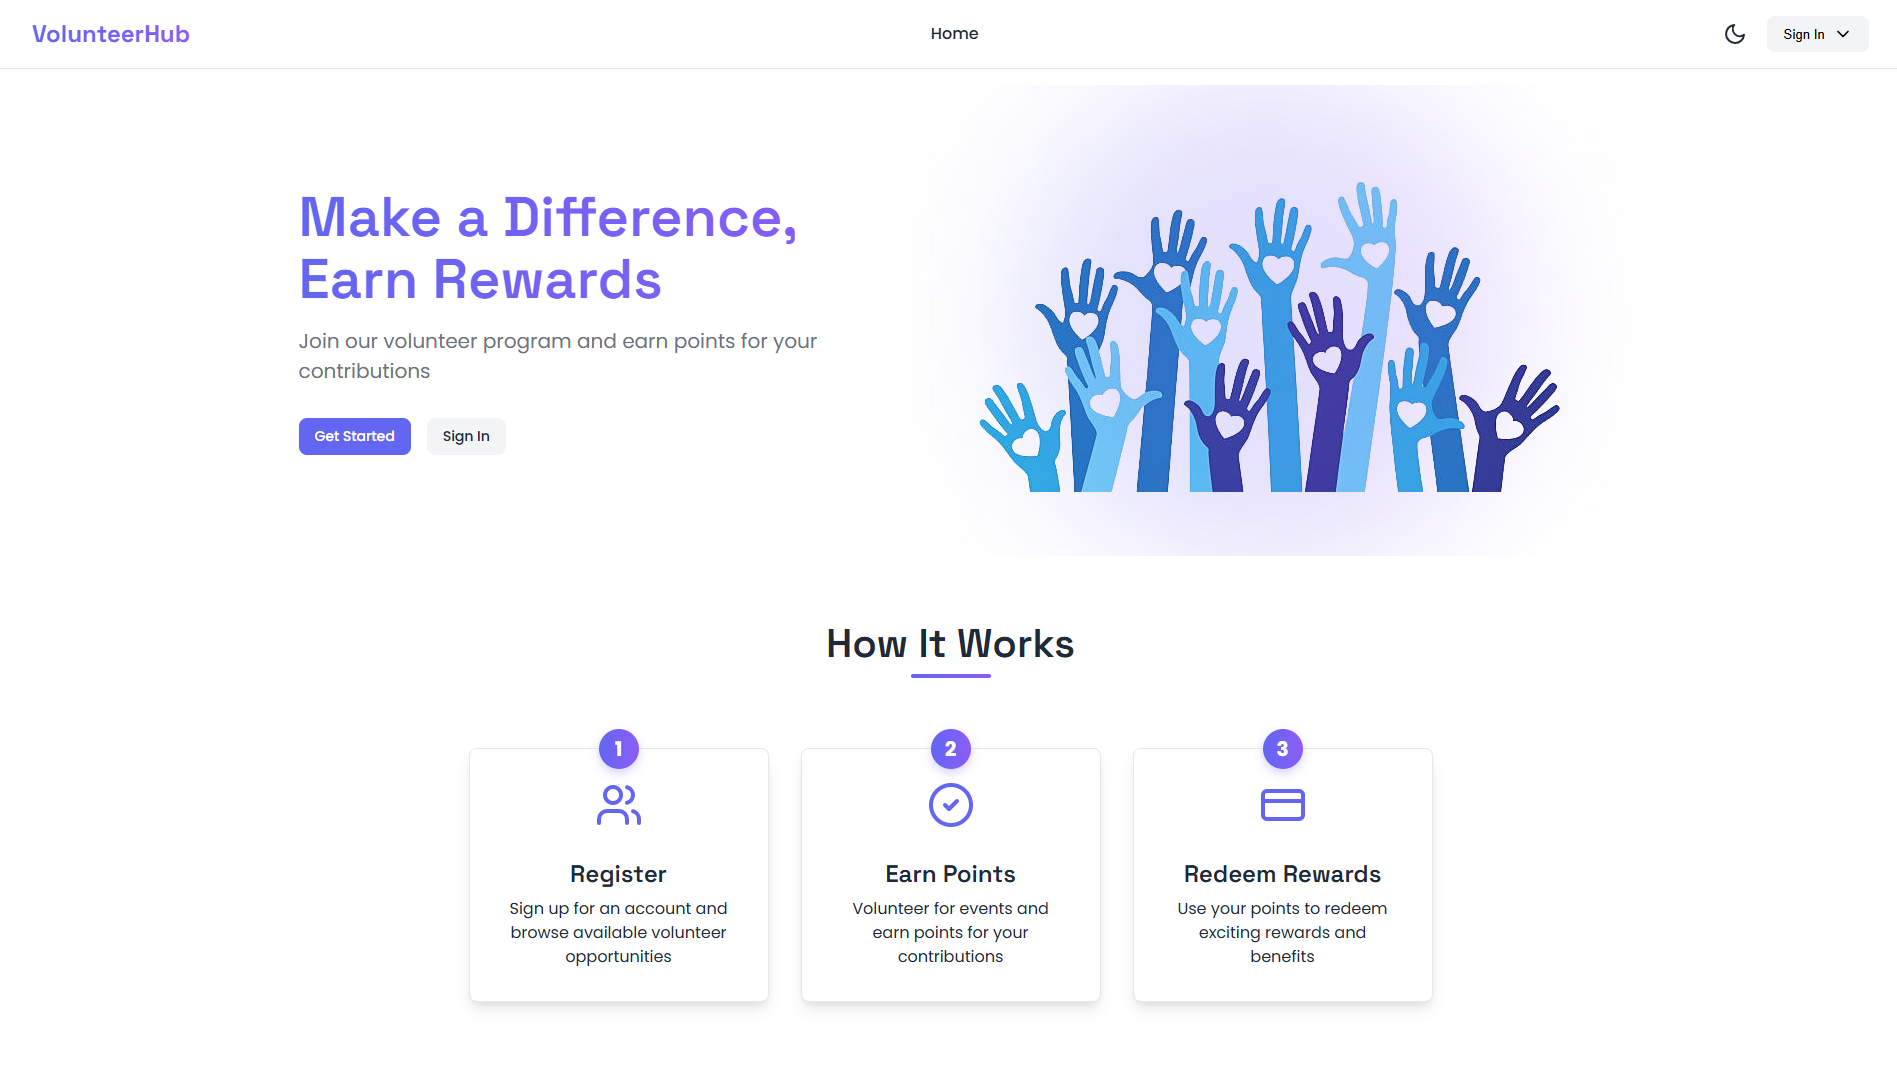
\includegraphics[width=1\textwidth]{home.png}
  \end{center}
\end{frame}

\begin{frame}{User Interface - Sign Up}
  \begin{center}
    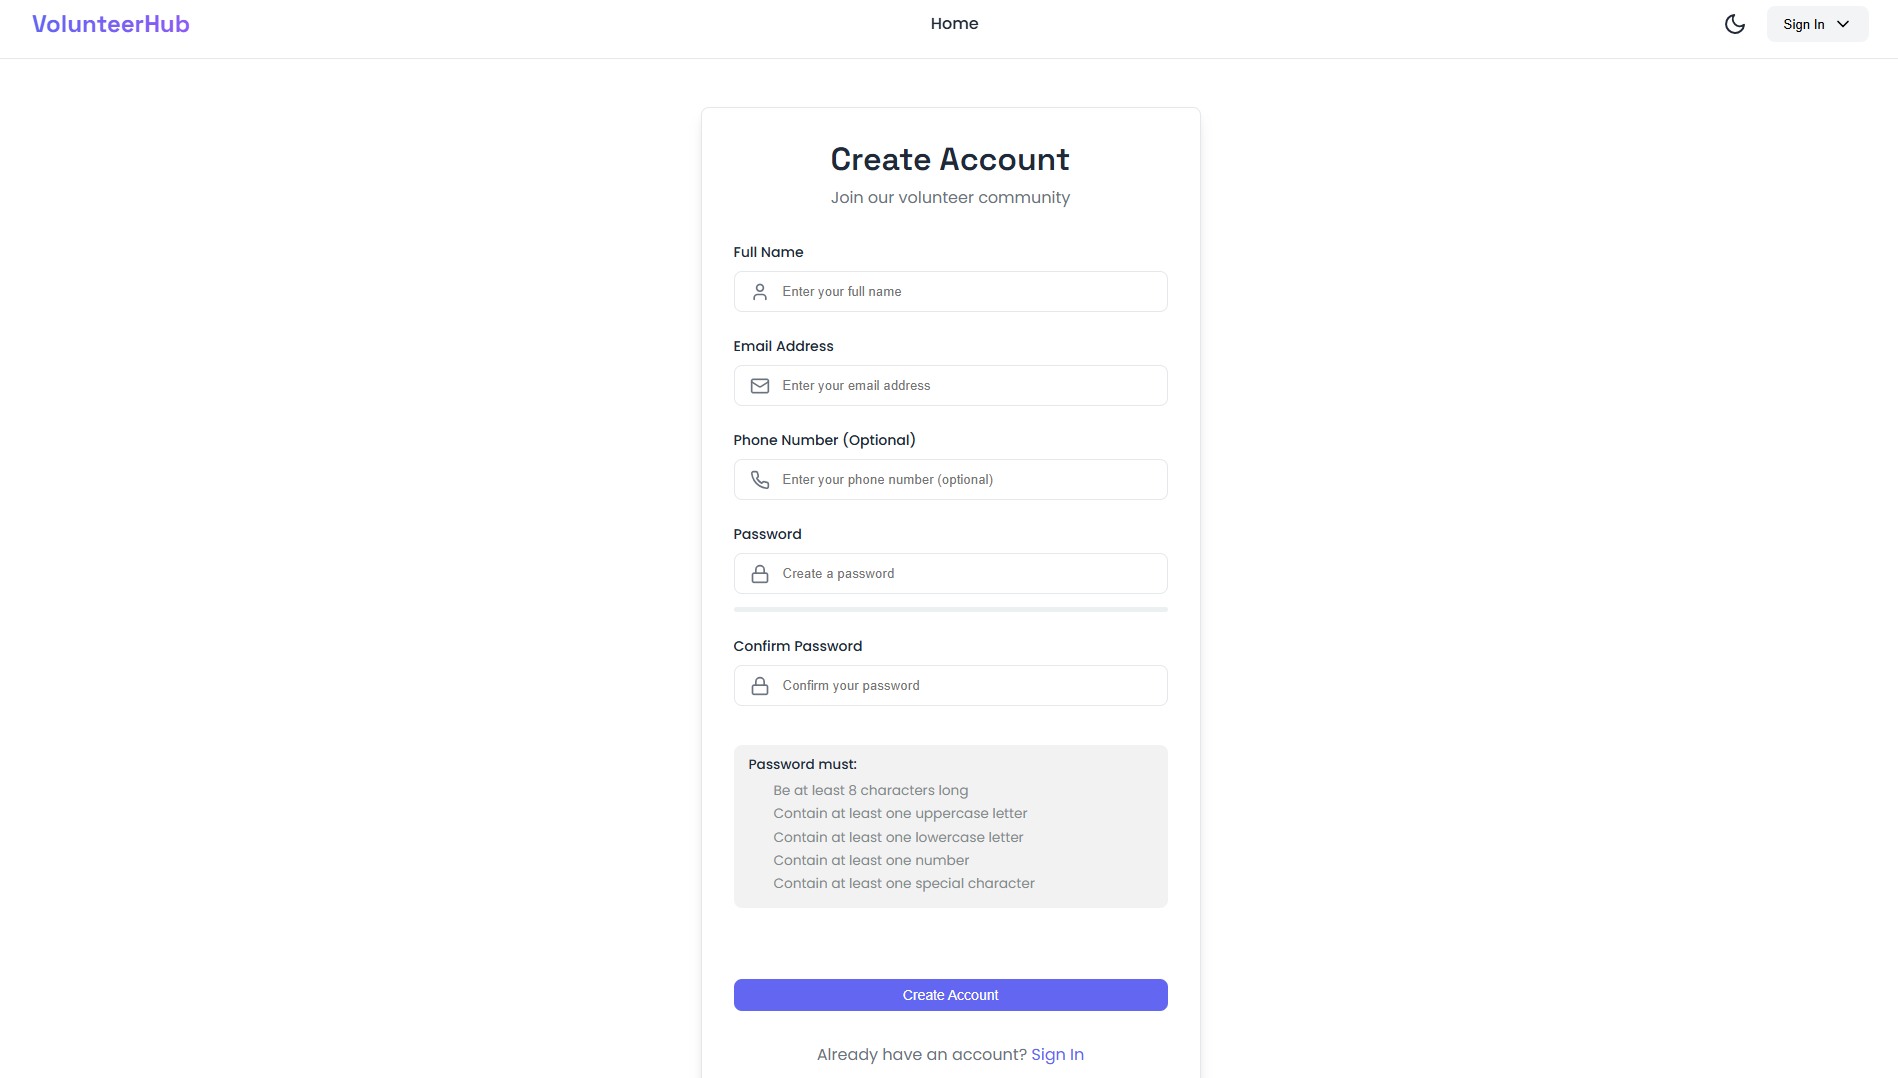
\includegraphics[width=1\textwidth]{sign_up.png}
  \end{center}
\end{frame}

\begin{frame}{User Interface - Sign In}
  \begin{center}
    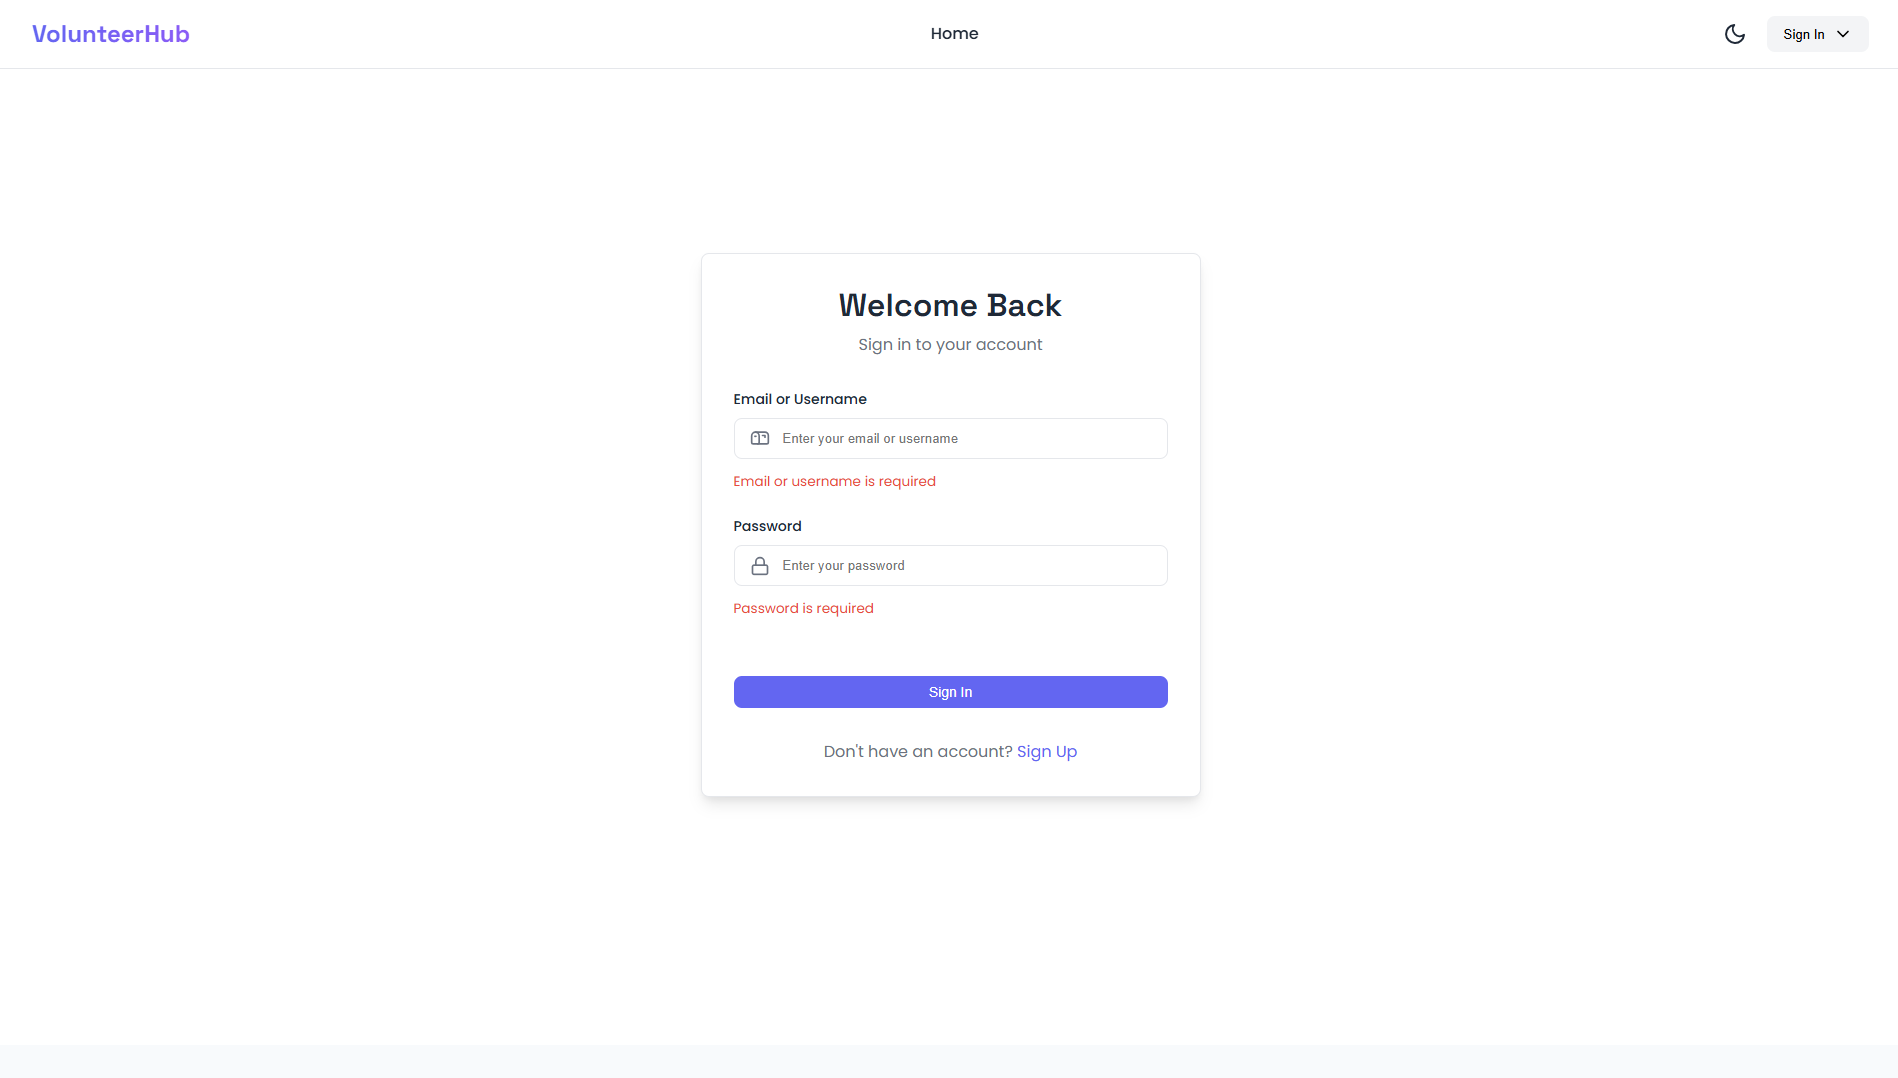
\includegraphics[width=1\textwidth]{sign_in.png}
  \end{center}
\end{frame}

\begin{frame}{User Interface - Admin Dashboard}
  \begin{center}
    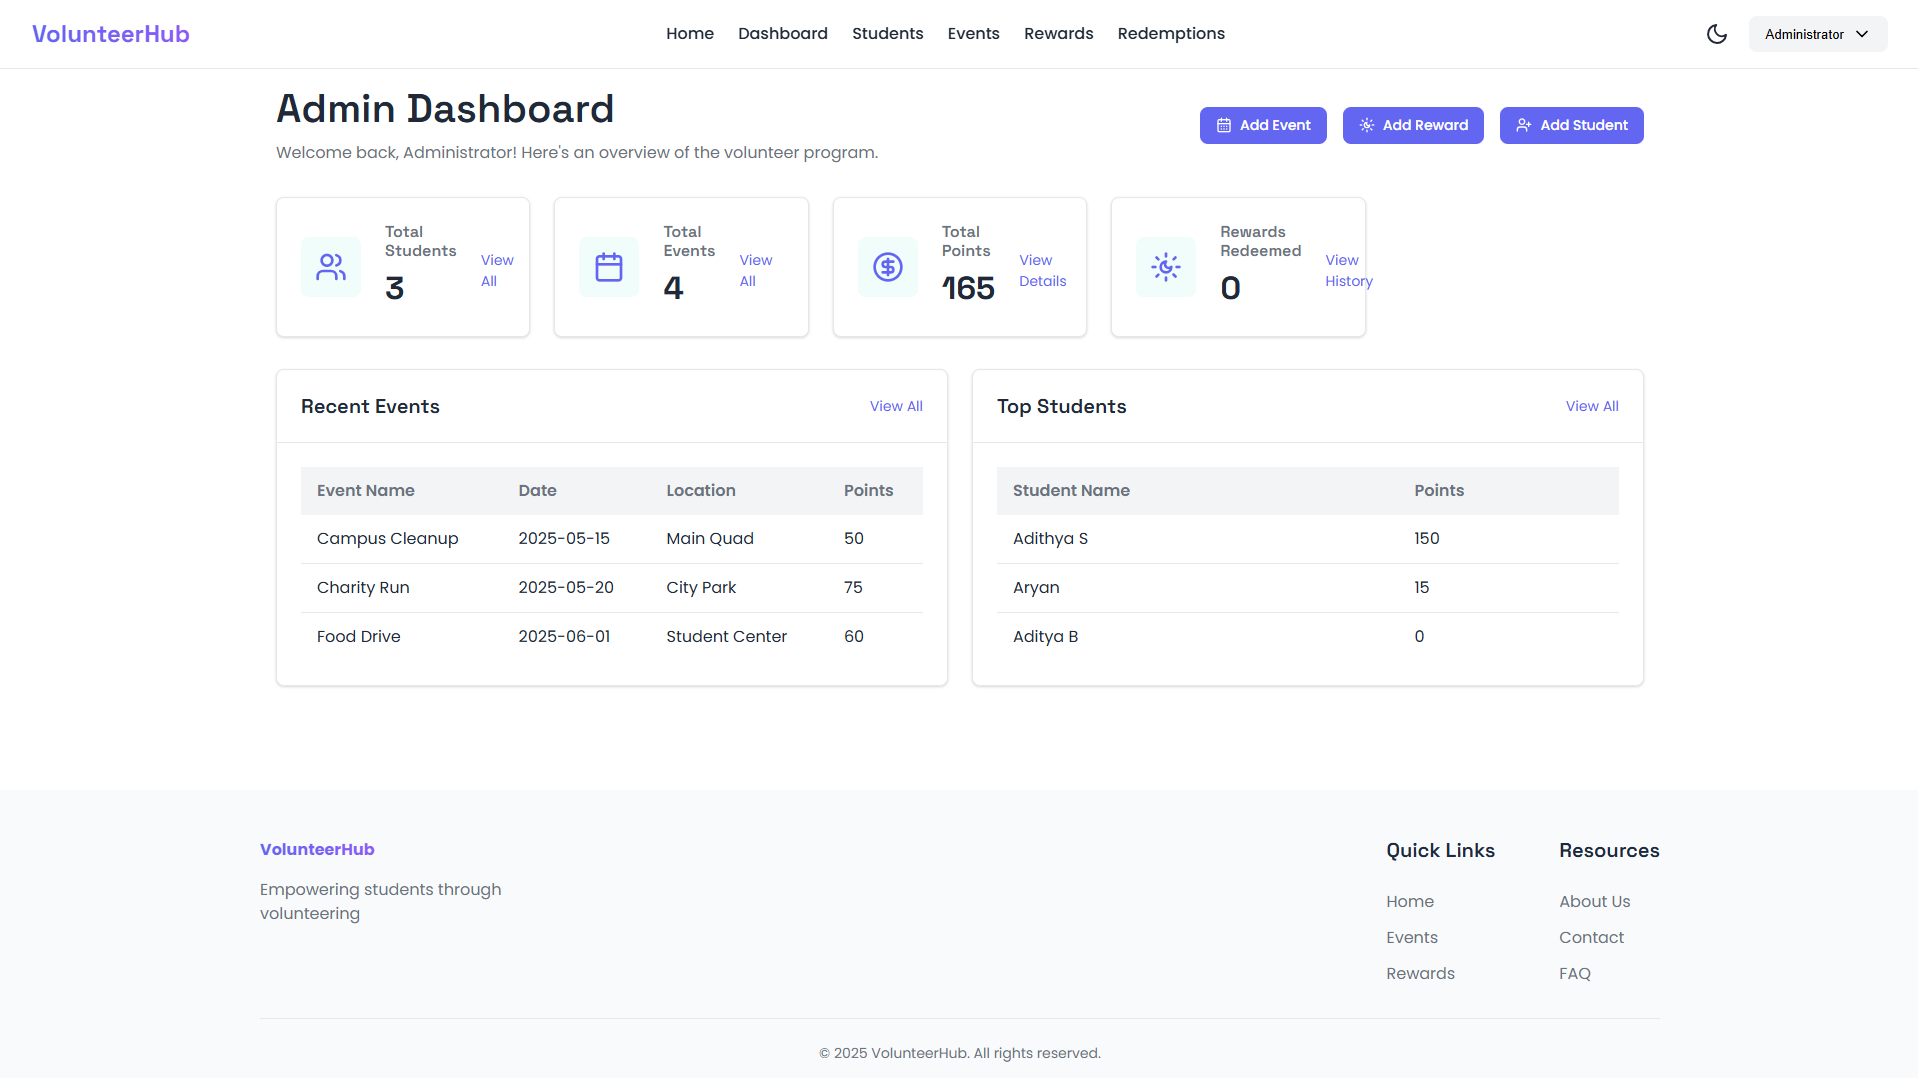
\includegraphics[width=1\textwidth]{admin_dashboard.png}
  \end{center}
\end{frame}

\begin{frame}{User Interface - Admin Student List}
  \begin{center}
    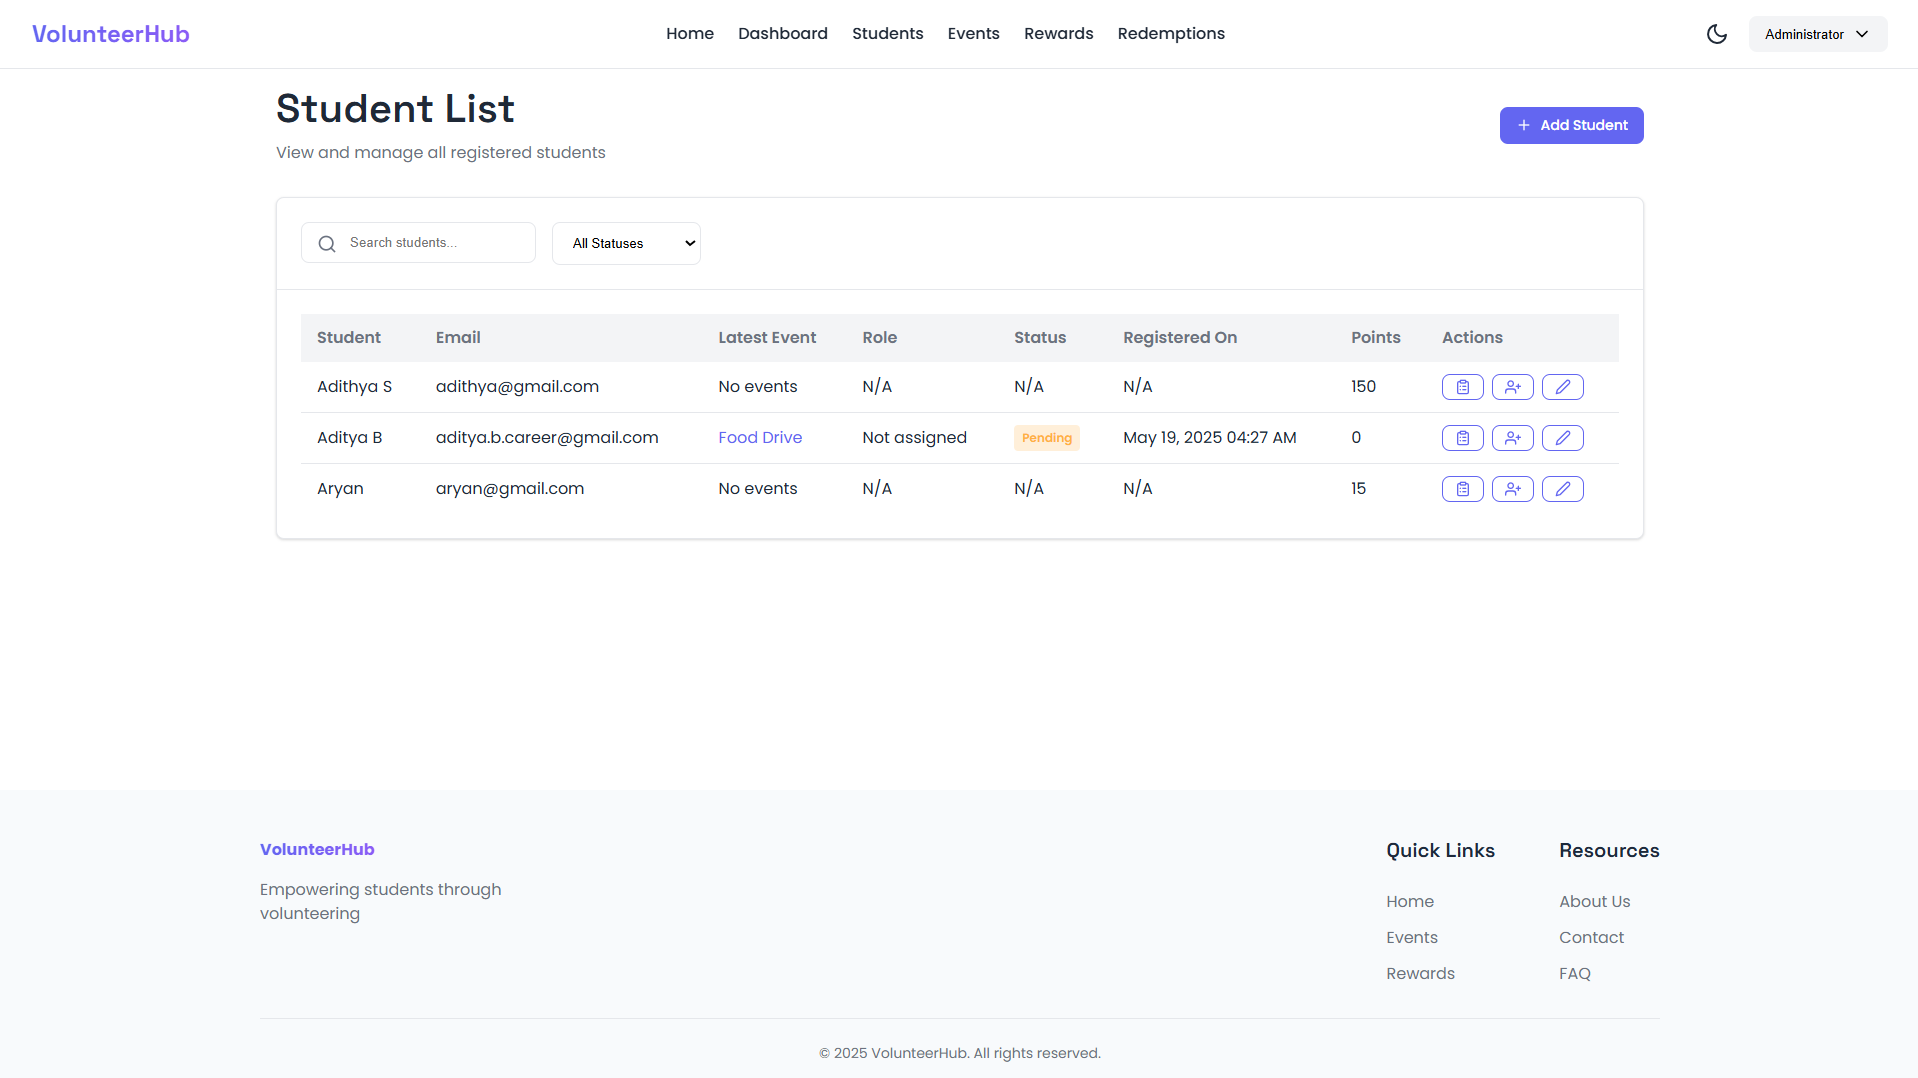
\includegraphics[width=1\textwidth]{admin_student_list.png}
  \end{center}
\end{frame}

\begin{frame}{User Interface - Admin Event Management}
  \begin{center}
    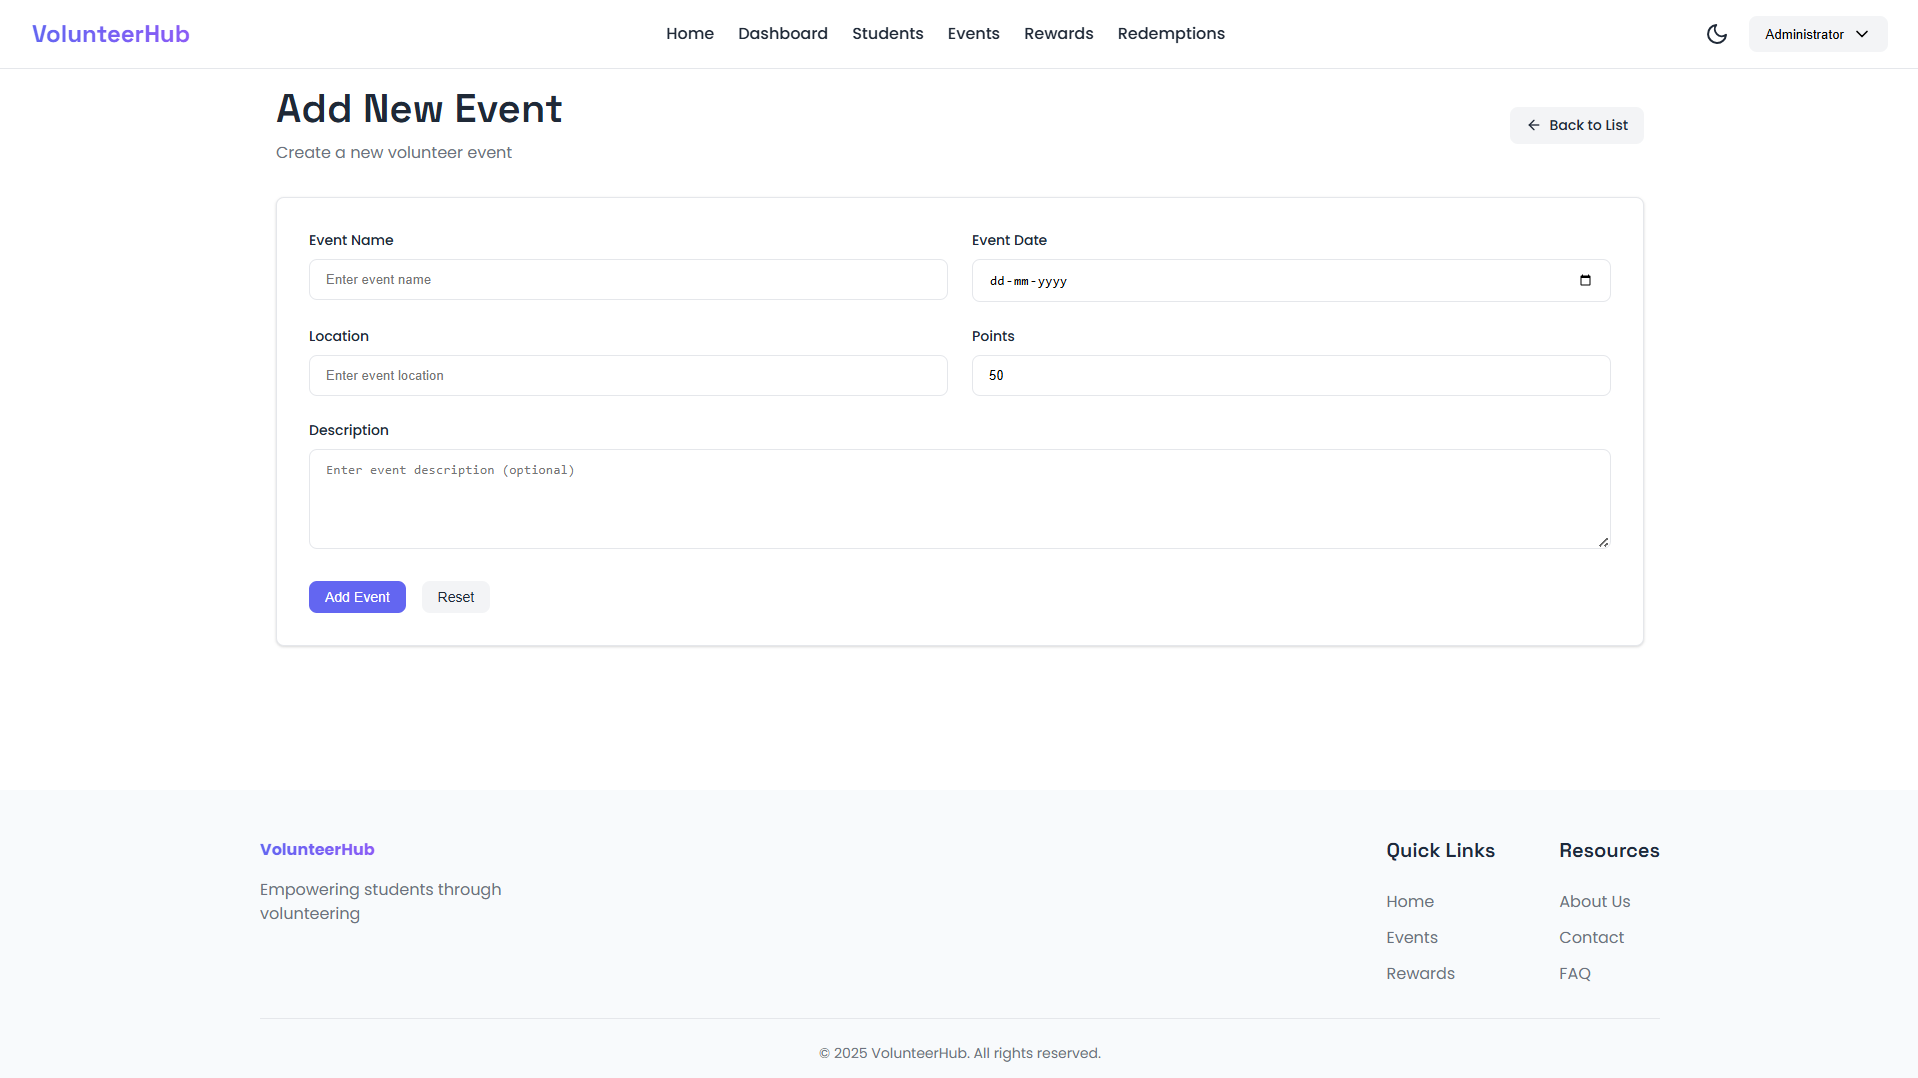
\includegraphics[width=1\textwidth]{admin_add_new_event.png}
  \end{center}
\end{frame}

\begin{frame}{User Interface - Admin Rewards System}
  \begin{center}
    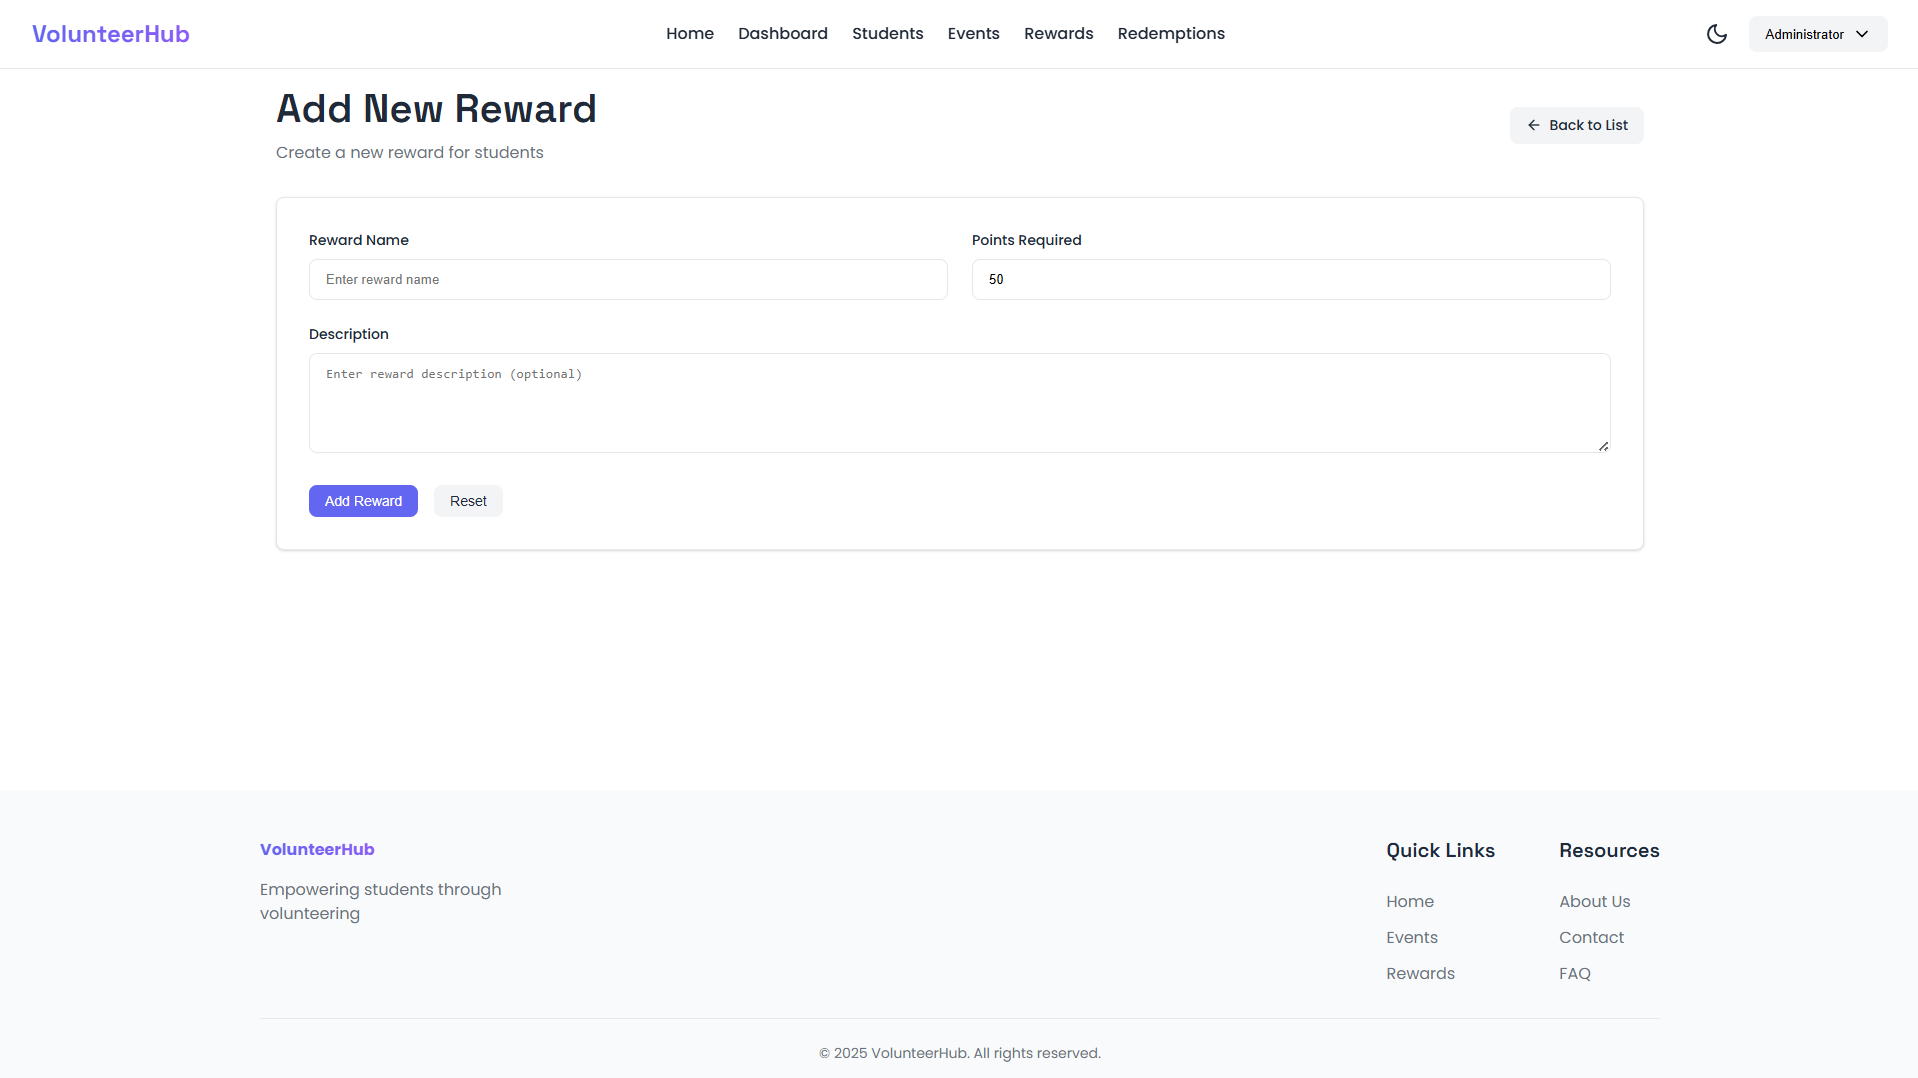
\includegraphics[width=1\textwidth]{admin_add_new_reward.png}
  \end{center}
\end{frame}

\begin{frame}{User Interface - Student Dashboard}
  \begin{center}
    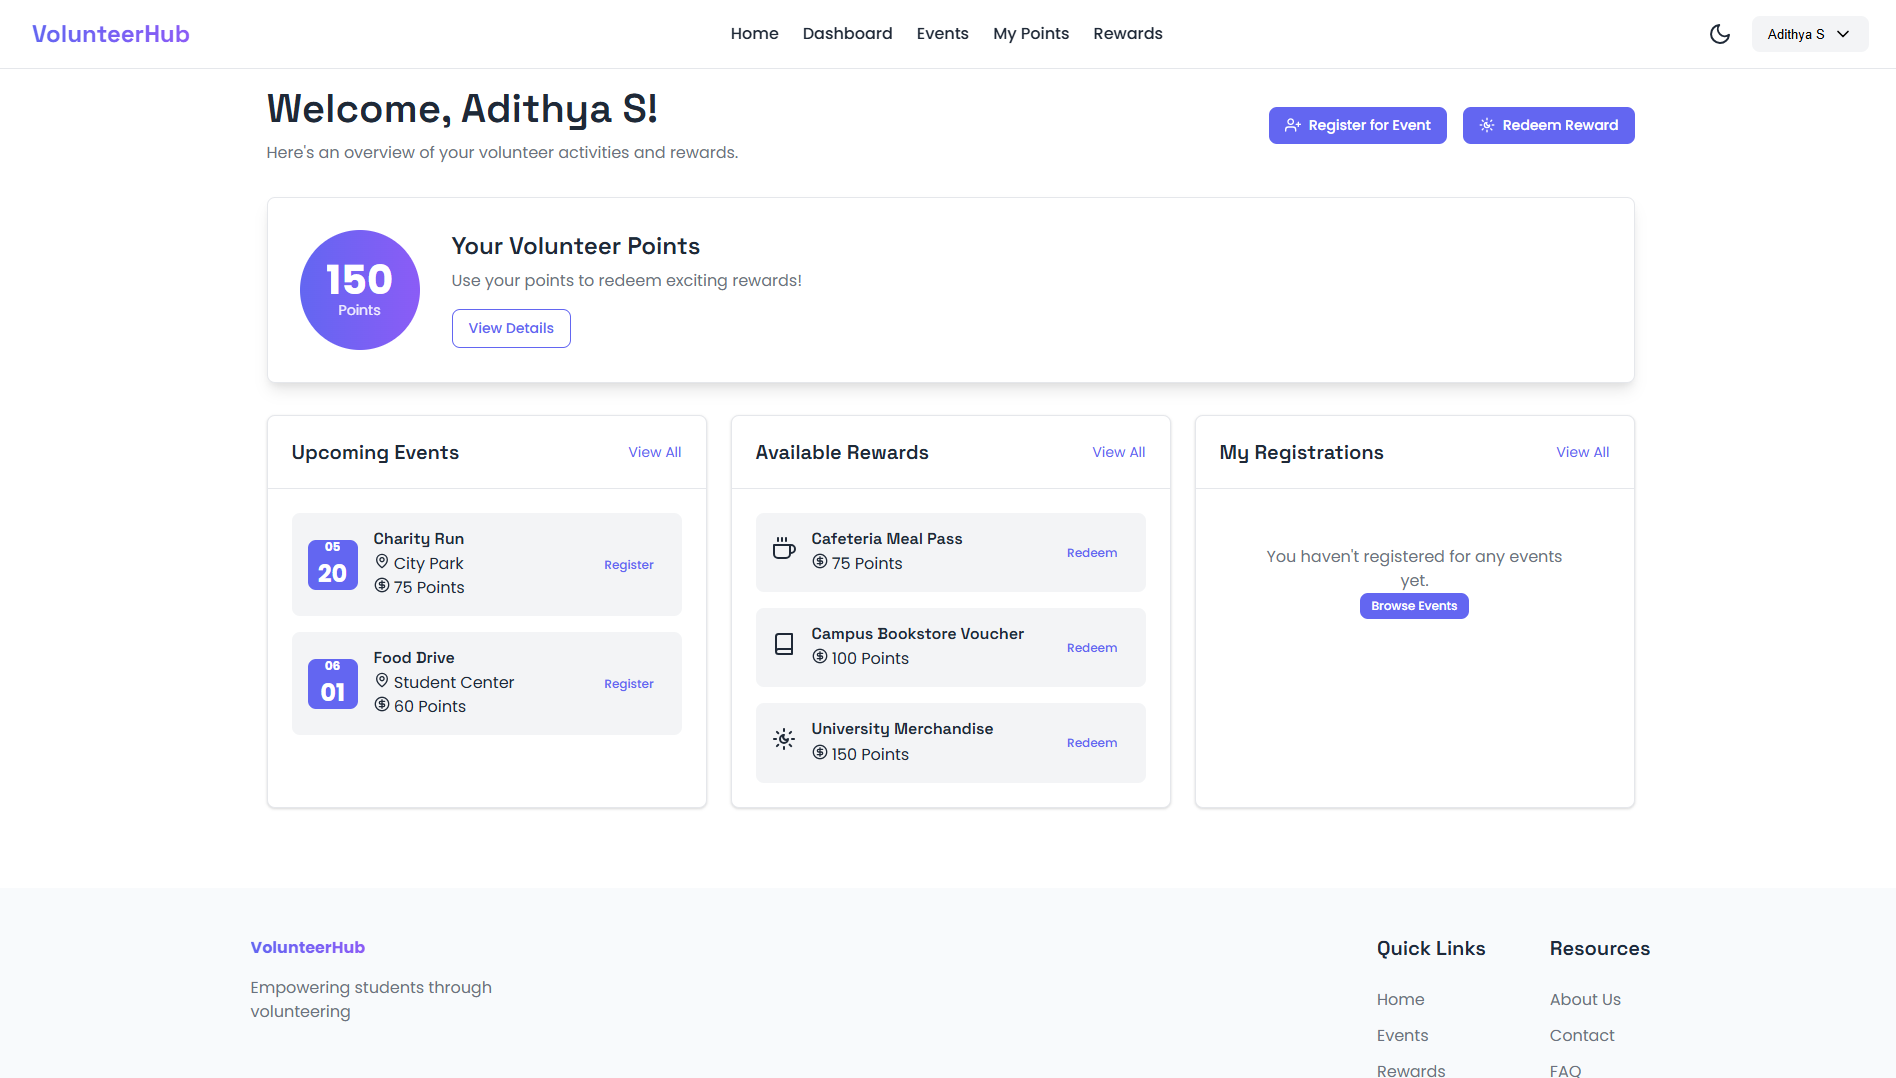
\includegraphics[width=1\textwidth]{Student_dashboard.png}
  \end{center}
\end{frame}

\begin{frame}{User Interface - Student Register}
  \begin{center}
    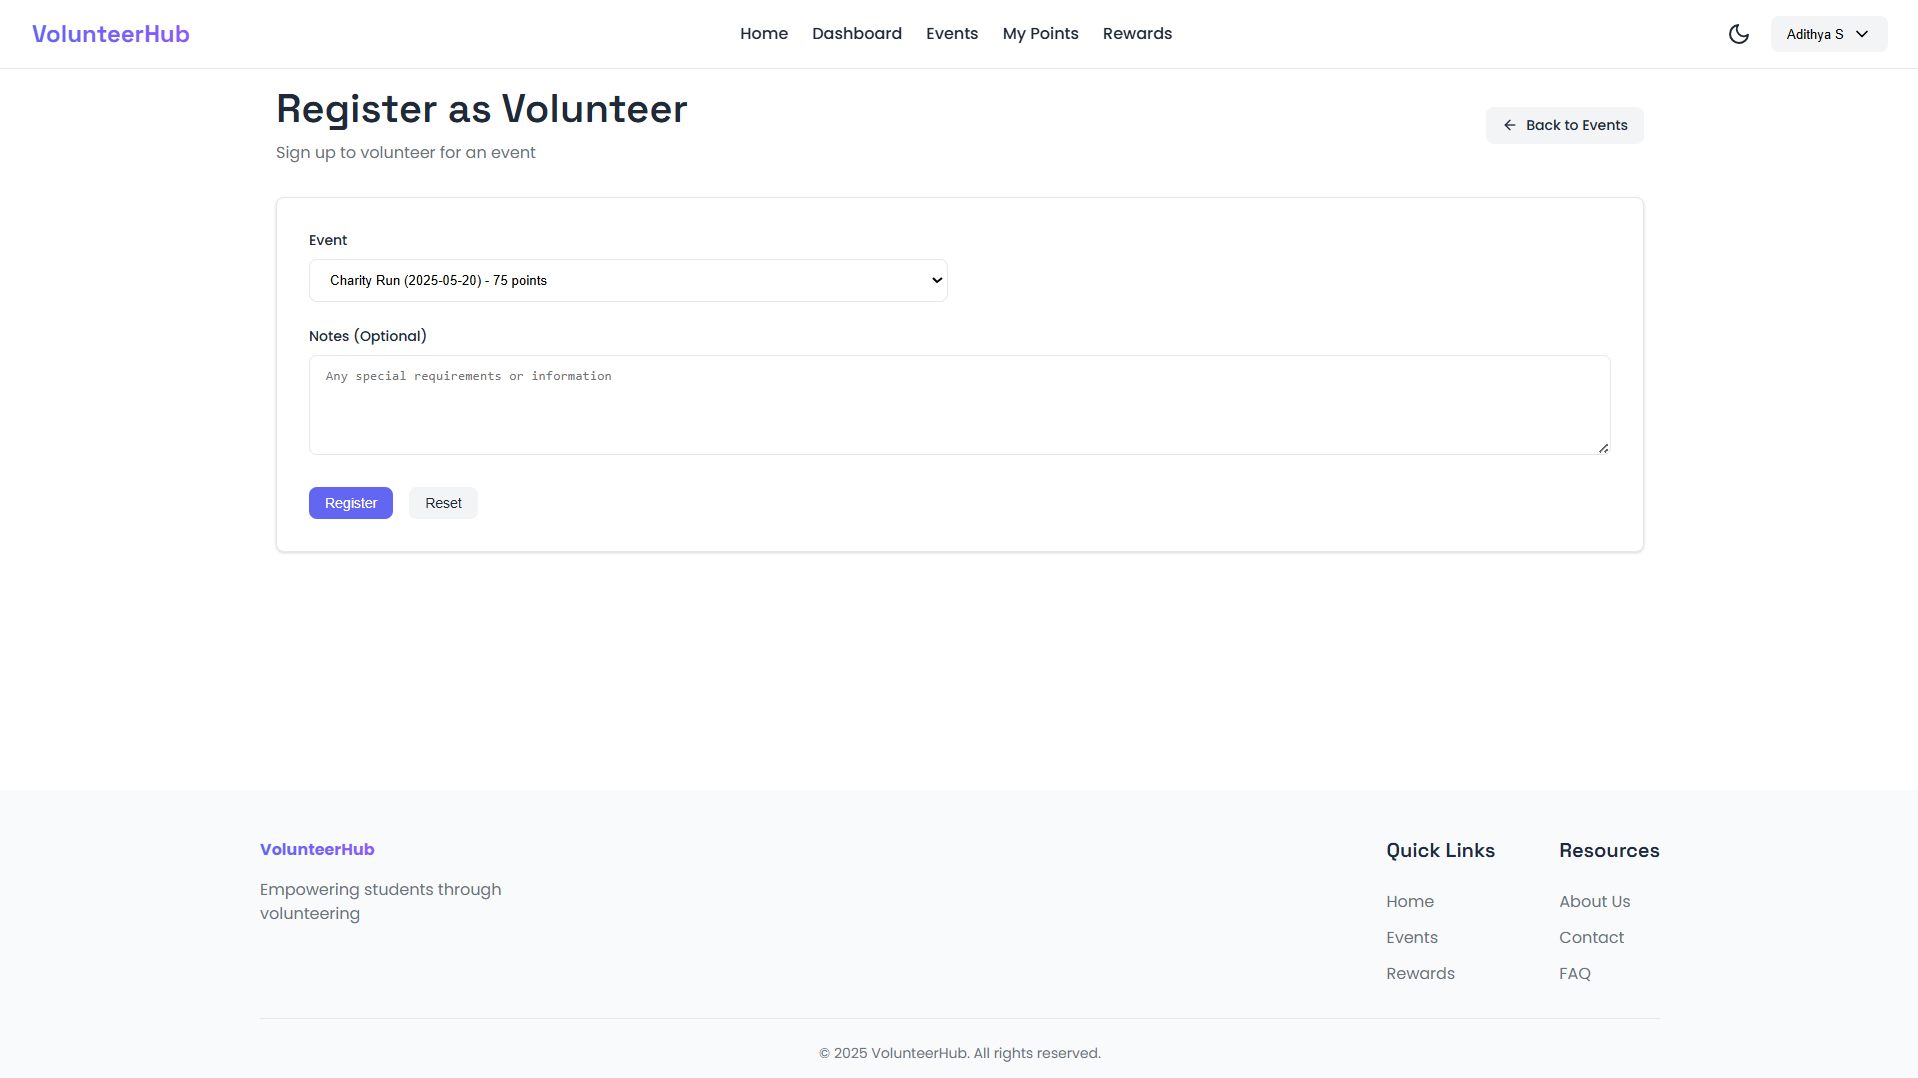
\includegraphics[width=1\textwidth]{Student_Registeer.png}
  \end{center}
\end{frame}

\begin{frame}{User Interface - Student Points Management}
  \begin{center}
    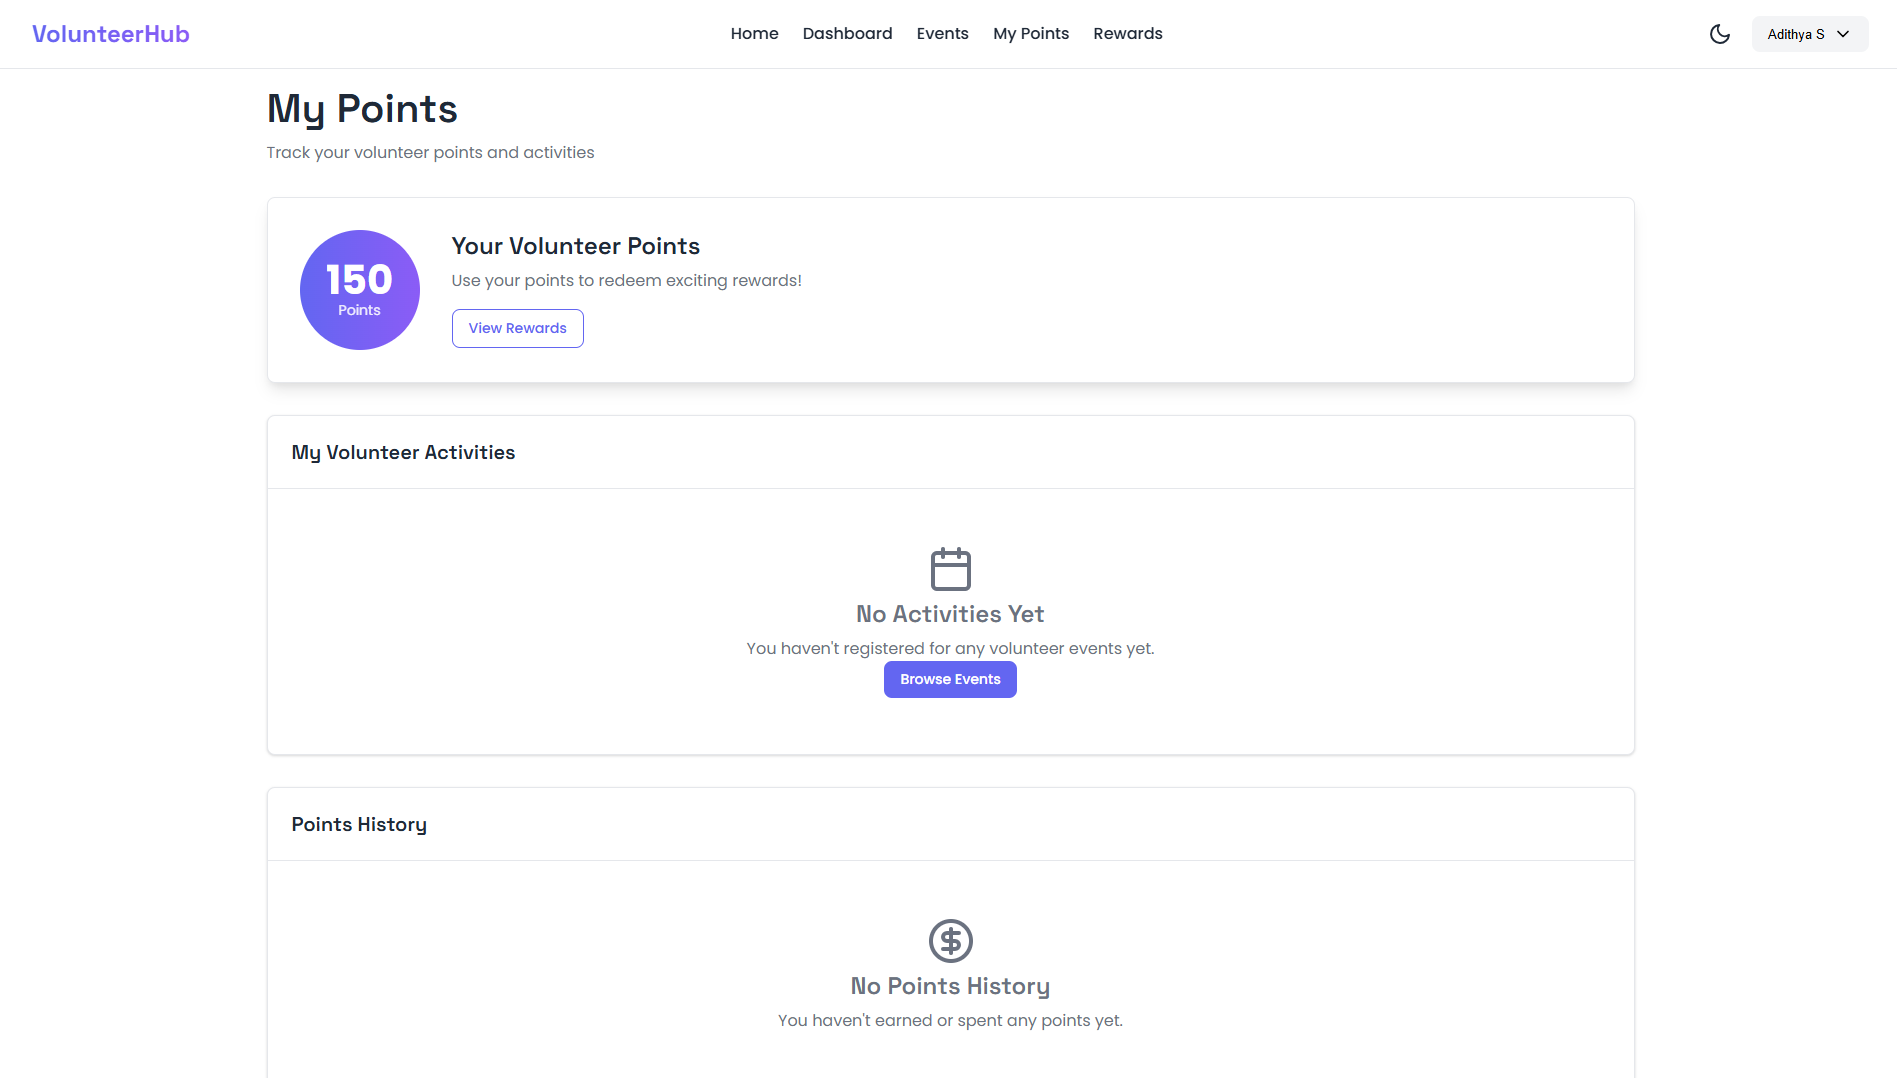
\includegraphics[width=1\textwidth]{Student_My_Points.png}
  \end{center}
\end{frame}

\begin{frame}{User Interface - Student Rewards System}
  \begin{center}
    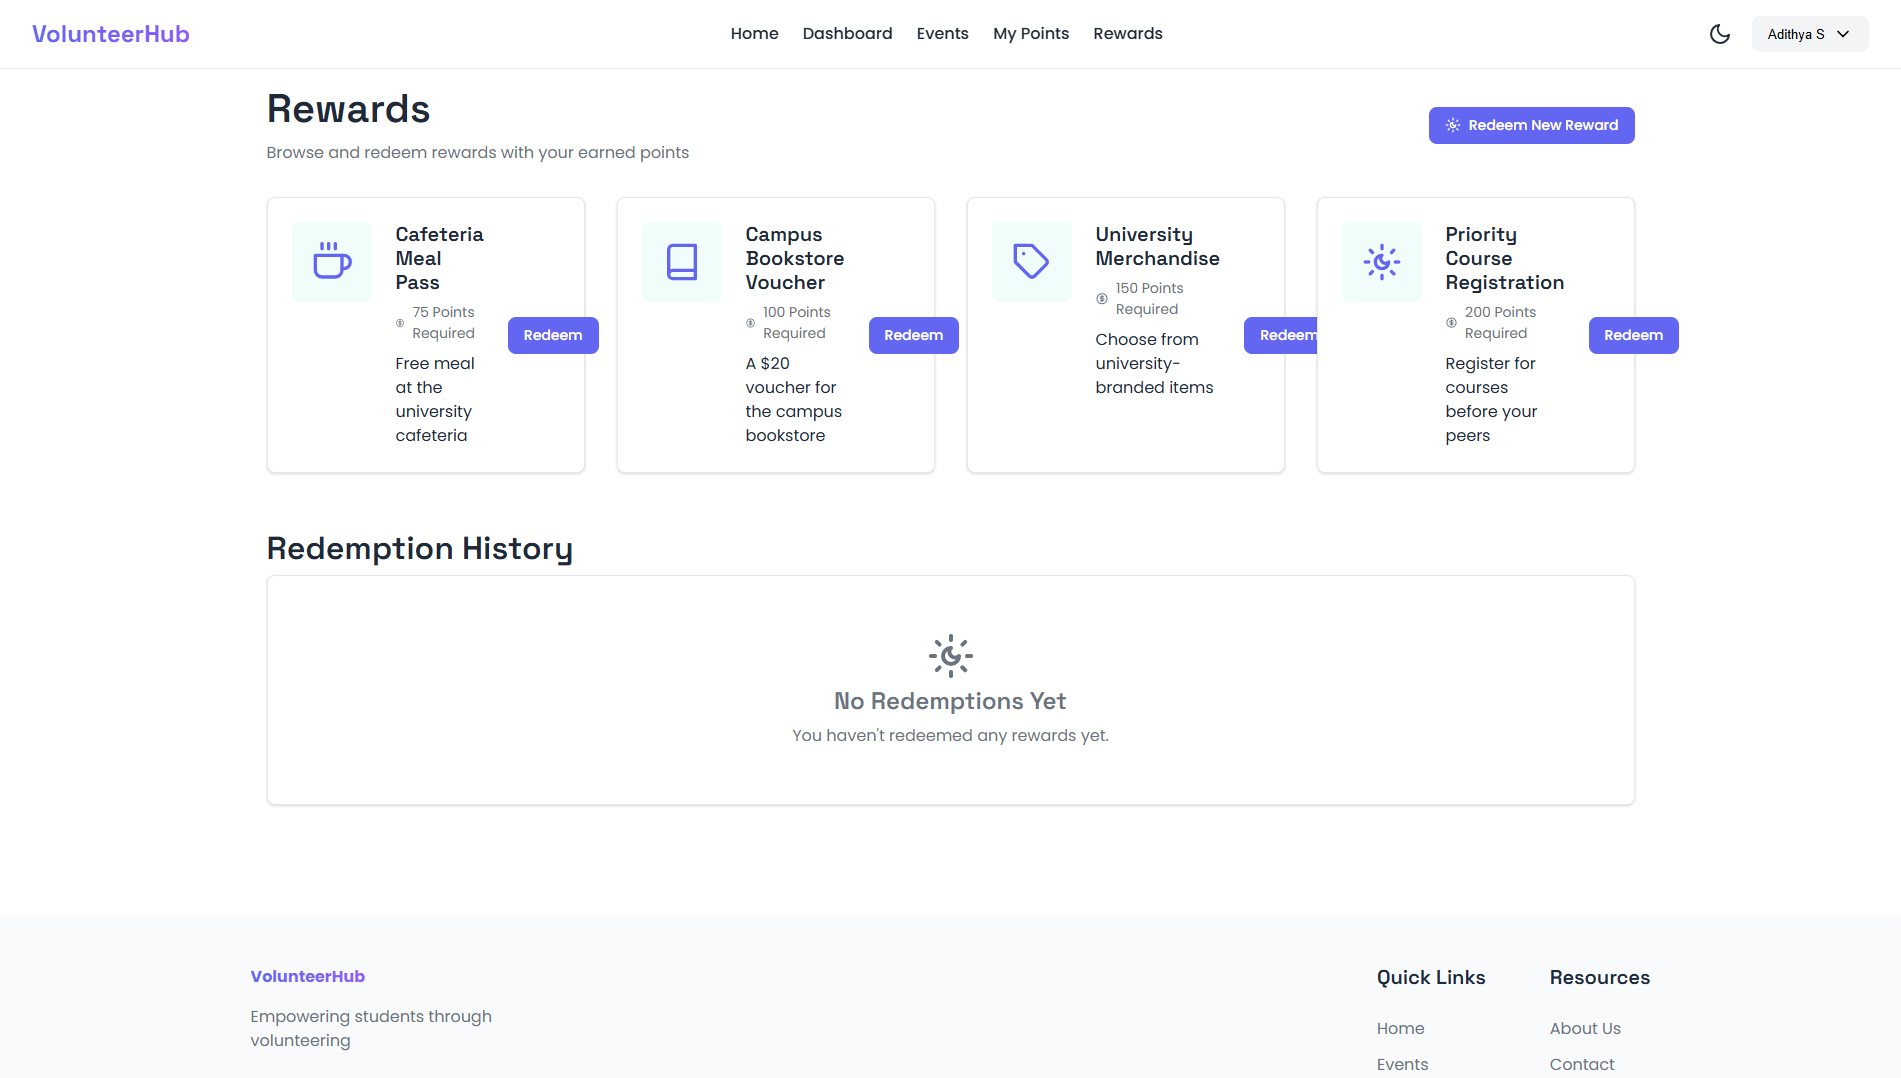
\includegraphics[width=1\textwidth]{student_Redeem_rewards.png}
  \end{center}
\end{frame}

\begin{frame}{User Interface - Student Rewards System}
  \begin{center}
    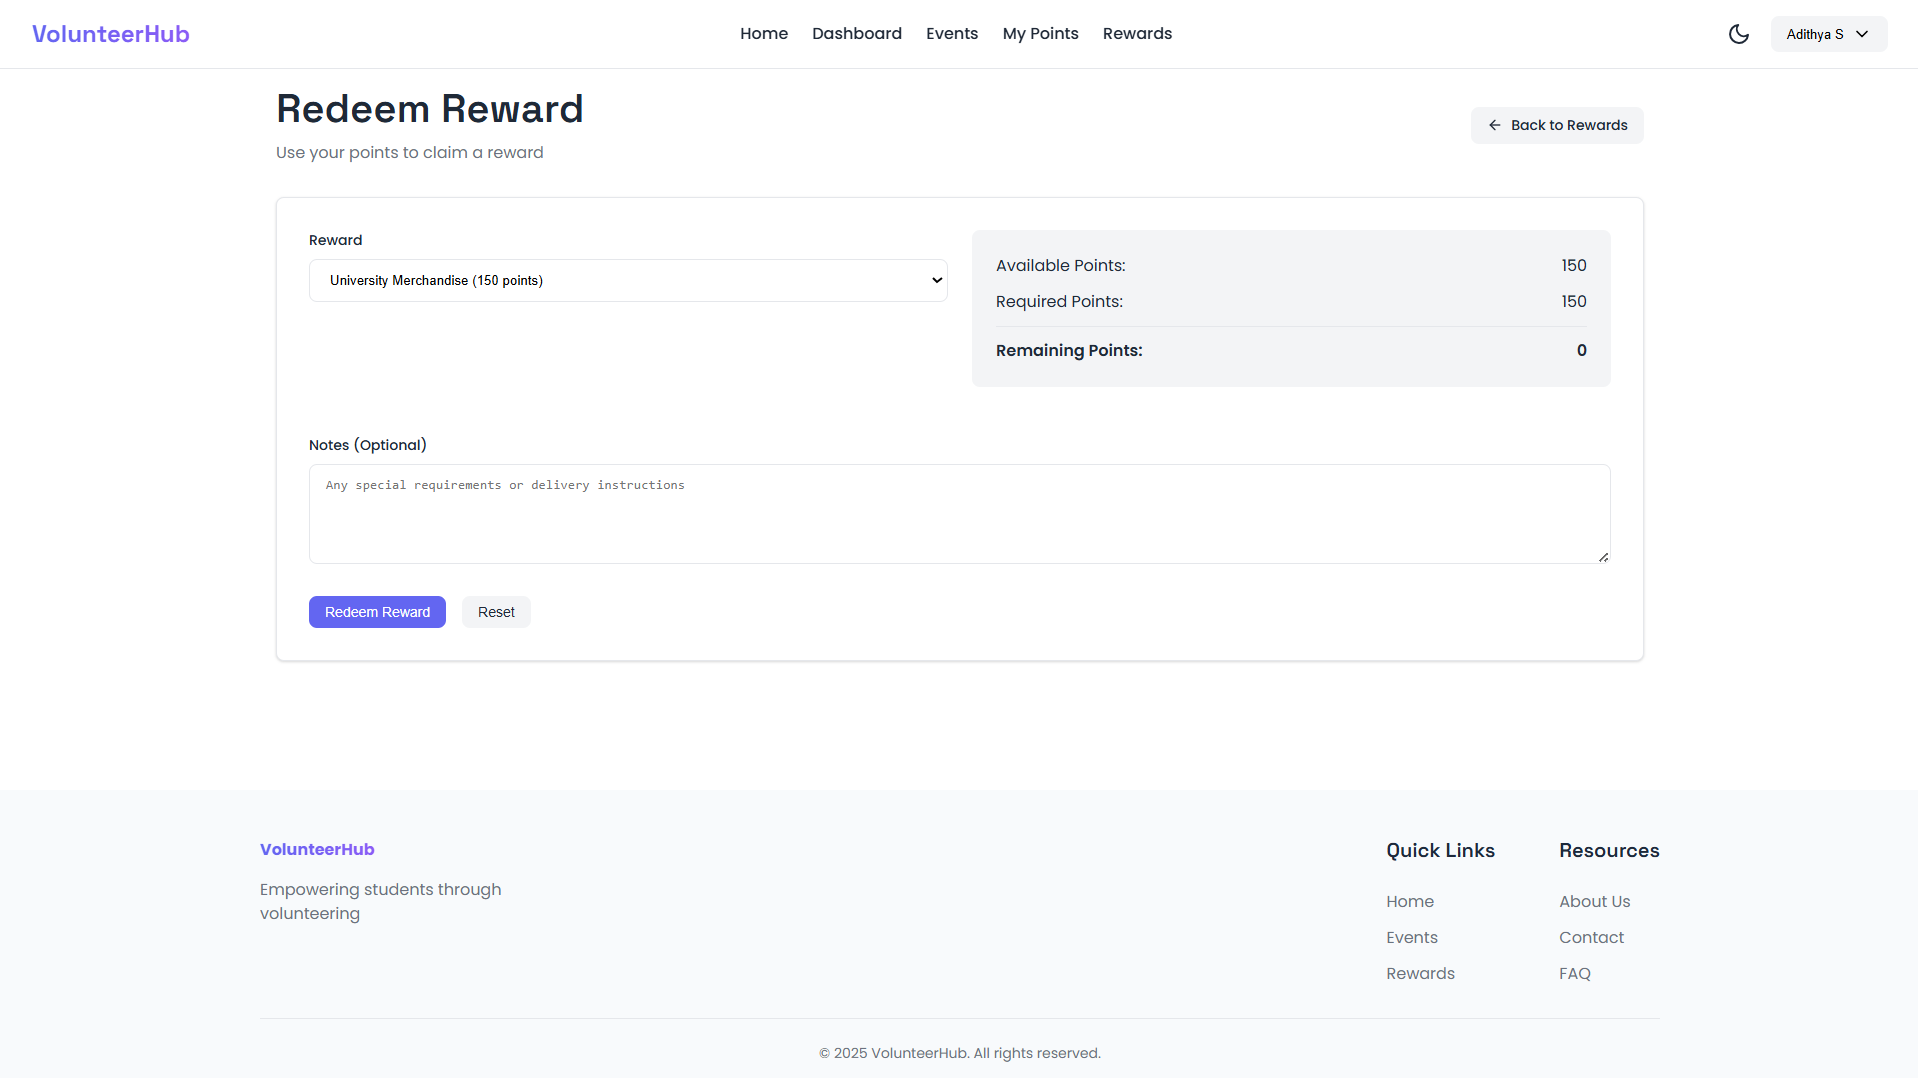
\includegraphics[width=1\textwidth]{student_Redeeming_Reward.png}
  \end{center}
\end{frame}

\section{Results/Conclusion}

\begin{frame}{Outcomes}
\setlength{\itemsep}{2pt}
  \begin{block}{Project Achievements}
    \begin{itemize}
      \item Implemented a full-featured volunteer management system
      \item Created an intuitive, responsive user interface
      \item Developed a secure points tracking and reward system
      \item Implemented comprehensive admin controls for event management
      \item Ensured data integrity with proper validation and constraints
    \end{itemize}
  \end{block}
  \vspace{-0.3em}
  \begin{block}{Key Learnings}
    \begin{itemize}
      \item Database design principles and normalization
      \item Web application security best practices
      \item Full-stack development with Flask
      \item User experience considerations in application design
      \item Points-based incentive system implementation
    \end{itemize}
  \end{block}
\end{frame}

\begin{frame}{Conclusion}
  \begin{itemize}
    \item VolunteerHub provides an efficient solution for managing volunteer activities
    \item The points-based system effectively incentivizes student participation
    \item The application successfully addresses the needs of both administrators and volunteers
    \item The system can be easily extended with additional features
    \item Potential future enhancements:
      \begin{itemize}
        \item Email notifications
        \item Mobile application
        \item Analytics dashboard with visualizations
        \item Integration with other campus systems
      \end{itemize}
  \end{itemize}
\end{frame}

\begin{frame}{References}
  \scriptsize
  \begin{thebibliography}{9}
    \bibitem{ieee1} S. Sharma and M. Dhiman, "A Comprehensive Review of Volunteer Management Systems: Challenges and Future Directions," \textit{IEEE Access}, vol. 9, pp. 127640-127653, 2021.
    
    \bibitem{ieee2} P. Kumar, R. Singh, and A. Tripathi, "BlockVMS: Blockchain-Based Volunteer Management System for Transparent Community Service," \textit{IEEE Transactions on Engineering Management}, vol. 70, no. 5, pp. 1766-1780, 2023.
    
    \bibitem{acm1} J. Wang, S. Li, and Y. Chen, "Gamification in Volunteer Engagement: A Systematic Review," in \textit{Proceedings of the 2022 ACM Conference on Human Factors in Computing Systems (CHI '22)}, pp. 1-15, 2022.
    
    \bibitem{acm2} M. Brown and K. Davis, "PointsWork: A Points-Based Incentive System for Student Volunteer Management," in \textit{Proceedings of the 2021 ACM Conference on Computer Supported Cooperative Work and Social Computing}, pp. 267-278, 2021.

    \bibitem{springer1} R. González-Pérez and A. García-Holgado, "Digital Platform for Volunteer Management: A Case Study in Higher Education," in \textit{Advances in Human-Computer Interaction: Proceedings of HCI International 2022}, Springer, Cham, pp. 189-204, 2022.
    
    \bibitem{tech} Flask Documentation, \url{https://flask.palletsprojects.com/}
    
    \bibitem{db} SQLite Documentation, \url{https://www.sqlite.org/docs.html}
    
  \end{thebibliography}
\end{frame}

\begin{frame}[plain]{Thank You}
  \begin{center}
    \Huge Thank You!
    
    \vspace{1cm}
    \Large Questions \& Feedback?
    
    \vspace{1.5cm}
    \normalsize
    \textit{VolunteerHub: A Volunteer Management System}\\
    DBMS Mini Project
  \end{center}
\end{frame}

\end{document}